% Phasor Lock-in EP Primer — pedagogical introduction for ML audience
% Compile: pdflatex phasor_lockin_ep_primer.tex && bibtex phasor_lockin_ep_primer && pdflatex phasor_lockin_ep_primer.tex && pdflatex phasor_lockin_ep_primer.tex

\documentclass[11pt]{article}
\usepackage{amsmath,amssymb,amsthm}
\usepackage{bm}
\usepackage{booktabs}
% \usepackage{enumitem}  % not available; using standard itemize
\usepackage[margin=1in]{geometry}
\usepackage{hyperref}
\usepackage{natbib}
\usepackage{tikz}
\usepackage{pgfplots}
\pgfplotsset{compat=1.16}
\usetikzlibrary{arrows.meta,decorations.pathmorphing,backgrounds,positioning,calc,patterns,fit}

% Color palette
\definecolor{holo}{RGB}{30,110,190}
\definecolor{antiholo}{RGB}{200,80,30}
\definecolor{probeC}{RGB}{40,140,90}
\definecolor{basinC}{RGB}{90,150,200}
\definecolor{badC}{RGB}{200,120,120}
\definecolor{axisgray}{RGB}{110,110,110}

% Macros
\newcommand{\R}{\mathbb{R}}
\newcommand{\C}{\mathbb{C}}
\newcommand{\T}{\mathbb{T}}
\newcommand{\im}{\mathrm{i}}
\newcommand{\dd}{\mathrm{d}}
\newcommand{\dt}{\Delta t}
\newcommand{\unitproject}{\mathrm{unit\_project}}
\DeclareMathOperator{\Real}{Re}
\DeclareMathOperator{\Imag}{Im}
\DeclareMathOperator{\Tr}{Tr}

\title{Lock-in Equilibrium Propagation for Phasor Networks:\\
A Primer}
\author{}
\date{}

\begin{document}
\maketitle

% Citation key mapping:
% \cite{scellier2017equilibrium} -- original EP
% \cite{laborieux2022holomorphic} -- holomorphic EP
% \cite{olin2021deep} -- deep phasor networks
% \cite{olin2023hyperdimensional} -- HD computing for oscillatory systems
% \cite{whittington2019theories} -- EP review
% \cite{krotov2016dense} -- dense associative memory
% \cite{millidge2022predictive} -- predictive coding
% \cite{ororbia2023brain} -- brain-inspired ML survey
% \cite{rumelhart1986learning} -- backpropagation
% \cite{scellier2018equivalence} -- EP/Recurrent BP equivalence

\begin{abstract}
Equilibrium propagation (EP) trains an energy-based network by contrasting two settled states \citep{scellier2017equilibrium}. This note introduces \emph{lock-in EP}, the variant needed when neurons are \emph{phasors} --- unit-modulus complex numbers living on a circle rather than real activations on a line \citep{olin2021deep}. We assume the reader knows vanilla EP and focus on the single thing that genuinely changes: the map from the nudge $\beta$ to the equilibrium state is no longer holomorphic. The prior-art Cauchy contour method (complex $\beta$ on a circle) reads only the holomorphic component and misses the anti-holomorphic part \citep{laborieux2022holomorphic}. The standard two-phase contrast with a static real $\beta$ \emph{does} give the correct gradient --- but requires two settles. The remedy is to drive $\beta$ as a small \emph{real cosine in time}, $\beta(t)=\varepsilon\cos(\omega_p t)$, and recover the gradient by lock-in demodulation at $\omega_p$ in a \emph{single settle}. We build the method up from the vanilla-EP picture, illustrate the settling dynamics, and defer the heavier proofs to appendices.
\end{abstract}

%======================================================================
\section{Vanilla EP in Two Paragraphs}\label{sec:vanilla}
%======================================================================

Standard neural networks are feedforward systems: given inputs and an internal state, a series of linear and nonlinear operations produces the output \citep{rumelhart1986learning}. Deeper layers have no influence on earlier ones; they are causally unconnected. To carry out credit assignment --- adjusting parameters to improve the output given its current value --- the feedforward network must be unrolled backwards so that cause and effect can be reversed. While effective, this backpropagation requires separate computational steps and full memory of the network's state, inputs, and outputs, and is not generally accepted as a biologically realistic model of learning \citep{ororbia2023brain}.

Equilibrium propagation (EP) was developed as an alternative that trains neural networks without a separate backward pass \citep{scellier2017equilibrium}. The core principle is to define a scalar energy function $E(\theta, s)$ on a network of components with bidirectional influences. For a network with state $s$ containing neuronal activations and parameters $\theta$ containing weights $W$, a Hopfield-like energy for layer $\ell$ is
\begin{equation}
E_\ell(\theta, s) = \frac{1}{2}\|s_\ell\|^2 - s_\ell^\top W_\ell s_{\ell+1},
\end{equation}
summed across layers to give a single scalar $E(\theta, s)$. Unlike a feedforward network, we cannot solve for $s$ in one pass; symmetric connections allow influences to propagate forward and backward across the entire network. Instead, given inputs clamped at the first layer, we iteratively solve an energy minimization through simulated time:
\begin{equation}
\frac{\dd s}{\dd t} = -\frac{\partial E}{\partial s}(\theta, s).
\end{equation}
Under Lyapunov conditions, the network descends to a fixed point $s_0^*(\theta)$, the \emph{free equilibrium}. A physical computing platform would compute this implicitly via energy relaxation in continuous time. The equivalence to recurrent backpropagation is established in \citep{scellier2018equivalence}.

The free equilibrium may not match a desired output $y$. A scalar cost $C(s,y)$ measures the distance to $y$, and the energy is augmented as
\begin{equation}
F(\theta, s, \beta) = E(\theta, s) - \beta\, C(s, y),
\end{equation}
where $\beta$ is a small scalar. The network now descends on $F$ to reach a \emph{nudged} fixed point $s_\beta^*$. The central result of EP proves that the gradient of a loss $L(\theta)$ can be found as a difference of values at the two fixed points:
\begin{equation}
\frac{\partial L}{\partial \theta} = \lim_{\beta \to 0} \frac{1}{\beta}\left[\frac{\partial E}{\partial \theta}\big(\theta, s_\beta^*\big) - \frac{\partial E}{\partial \theta}\big(\theta, s_0^*\big)\right].
\end{equation}
(Note the minus sign: increasing $\beta$ lowers the energy toward the target. This convention matches the phasor energy in Eq.~\ref{eq:phasor-energy} and the implementation.)
By stepping through successive free and nudged equilibria, the network dynamics themselves express the information necessary to descend a loss function --- no separate backward pass required.

%======================================================================
\section{Phasor Energy, Descent, and Settling}\label{sec:energy-cost}
%======================================================================

\subsection{Phase Energy Functions}\label{ssec:phase-energy}

Three substitutions map vanilla EP onto the phasor domain (Figure~\ref{fig:statespace}):

\begin{table}[ht]
\centering
\caption{Vanilla EP $\to$ Phasor EP: three substitutions.}
\label{tab:three-subs}
\begin{tabular}{@{}lll@{}}
\toprule
Vanilla EP & Phasor EP & What changes \\
\midrule
State $s \in \R^n$ & $z \in \T^n = \{z\in\C^n : |z_j|=1\}$ & Topological saturation replaces squashing \\
Coupling $s^\top W s$ & $\Real\langle W z_{\ell-1}, z_\ell \rangle$ & Cosine similarity = relative phase \\
Cost $\|s-y\|^2$ & $1 - \frac{1}{d}\Real\langle z_L, y \rangle$ & Pull toward target on the circle \\
\bottomrule
\end{tabular}
\end{table}

A phasor network of $L$ layers has hidden state $z_\ell \in \T^{d_\ell} \subset \C^{d_\ell}$ on the torus $\T^{d_\ell} = \{z\in\C^{d_\ell} : |z_j|=1 \text{ for all } j\}$, real weight matrices $W_\ell \in \R^{d_\ell \times d_{\ell-1}}$, and per-channel oscillator eigenvalues $k_\ell = \lambda_\ell + \im\omega_\ell$ with $\lambda_{\ell,c} < 0$ \citep{olin2021deep}. The input $x = z_0$ is fixed and the dynamics are constrained to the torus by the entrywise \emph{unit projector}
\begin{equation}
\unitproject(g) = \frac{g}{|g|}, \qquad g \in \C \setminus \{0\}.
\end{equation}

Following our prior work, we start by considering a network of frequency-locked oscillators which produce a vector of complex states $z$ representing the phase of each oscillator with respect to a reference \citep{olin2021deep,olin2023hyperdimensional}. The same cosine-similarity metric used to calculate the ``closeness'' of two phase vectors applies directly as the scalar energy for a single layer:
\begin{equation}\label{eq:phasor_layer_energy}
\Phi_\ell = \Real\langle W_\ell z_{\ell-1}, z_\ell \rangle,
\end{equation}
where cosine similarity in the complex plane is the real component of the Hermitian inner product between the weighted drive from the previous layer ($W_\ell z_{\ell-1}$) and the layer's current state ($z_\ell$). Similarly, the cost at the output uses the same metric:
\begin{equation}\label{eq:phasor-cost}
C(z_L, y) = 1 - \frac{1}{d}\Real\langle z_L, y \rangle,
\end{equation}
where $z_L$ is the network's output layer of $d$ oscillators and $y$ is the desired output expressed in relative phases on the same domain. The Hamiltonian energy for the entire network is then
\begin{equation}\label{eq:phasor-energy}
\Phi = \sum_{\ell=1}^L \Real\langle W_\ell z_{\ell-1}, z_\ell \rangle \;-\; \beta\, C(z_L, y).
\end{equation}

\subsection{Energy Gradient on the Torus}\label{ssec:energy-gradient}

To descend $\Phi$, we need its gradient with respect to the phasor states. Because $z$ lives on the unit torus, we use Wirtinger calculus: the gradient with respect to $\bar{z}_\ell$ (the covector on the tangent space of $\T^{d_\ell}$) gives the drive into layer $\ell$ \citep{laborieux2022holomorphic}. One can show (see \S\ref{sec:liep_proof} for the full derivation) that the energy gradient contains only the coupling terms:
\begin{align}
\frac{\partial \Phi}{\partial \bar{z}_\ell} &= W_\ell z_{\ell-1} + W_{\ell+1}^\top z_{\ell+1}, \qquad \ell = 1,\dots,L-1, \label{eq:grad-hidden}\\
\frac{\partial \Phi}{\partial \bar{z}_L} &= W_L z_{L-1} + \frac{\beta}{d}\, y. \label{eq:grad-output}
\end{align}
The energy $\Phi$ has no self-interaction term; the decay (self-force) comes from the oscillator dynamics, not from $\Phi$.

\subsection{Continuous Gradient Flow with Decay}\label{ssec:continuous-flow}

To ensure the gradient flow converges to a stable fixed point, we add a linear decay term $-\gamma z_\ell$ (with $\gamma > 0$) to the energy gradient. This is not derived from $\Phi$; it is a design choice that makes the continuous dynamics Lyapunov-stable. The continuous-time flow becomes
\begin{equation}\label{eq:continuous-flow}
\frac{\dd z_\ell}{\dd t} = -\gamma z_\ell - \frac{\partial \Phi}{\partial \bar{z}_\ell}
= -z_\ell + W_\ell z_{\ell-1} + W_{\ell+1}^\top z_{\ell+1},
\qquad \ell = 1,\dots,L,
\end{equation}
where we set $\gamma = 1$ and $W_{L+1}^\top z_{L+1} \equiv \frac{\beta}{d}\, y$ at the output layer. This flow lives in the ambient complex space $\C^{d_\ell}$; it does not by itself preserve $|z_{\ell,j}|=1$. The term $-z_\ell$ is a stabilizing decay; the coupling terms pull $z_\ell$ toward the feedforward drive $W_\ell z_{\ell-1}$ and the feedback $W_{\ell+1}^\top z_{\ell+1}$. This matches the EP gradient flow \citep{scellier2017equilibrium}.

\subsection{Projection onto the Torus}\label{ssec:projection}

To enforce the topological constraint $|z_{\ell,j}|=1$, we project the velocity onto the tangent space of the torus at each step. The tangent space at $z \in \T^n$ is
\begin{equation}
T_z\T^n = \{ v \in \C^n : \Real(\bar{z}_j v_j) = 0 \text{ for all } j \},
\end{equation}
i.e., the velocity must be phase-orthogonal to the state (purely rotational). This geometric view connects to optimization on manifolds \citep{olin2021deep}. Projecting the continuous flow onto this tangent space and discretizing with step $\dt$ yields the \emph{projected Euler} update (textbook form)
\begin{equation}\label{eq:discrete-settle-textbook}
z_\ell \;\leftarrow\; \unitproject\Big( z_\ell + \dt\big( -z_\ell + W_\ell z_{\ell-1} + W_{\ell+1}^\top z_{\ell+1} \big) \Big),
\qquad \ell = 1,\dots,L,
\end{equation}
where the unit projector $\unitproject(g) = g/|g|$ normalizes each component back to the unit circle.

The implementation in \texttt{src/ep.jl} (\texttt{\_project\_damp}) uses a mathematically equivalent but numerically fused form:
\begin{equation}\label{eq:discrete-settle-impl}
z_\ell \;\leftarrow\; (1-\dt)\,z_\ell + \dt \;\unitproject\Big( -z_\ell + W_\ell z_{\ell-1} + W_{\ell+1}^\top z_{\ell+1} \Big).
\end{equation}
This is a convex combination of the old state and the projected drive. The two forms are equivalent to $O(\dt)$ (both are consistent first-order integrators for the constrained gradient flow on $\T^n$) but differ at finite $\dt$. The fused form is preferred because it is a single broadcast pass (no temporaries), bit-identical on CPU/GPU, and the decay $(1-\dt)z$ is explicit and stable. This form is used in all experiments \citep{olin2021deep}.

\subsection{Fixed Point Interpretation}\label{ssec:fixed-point}

At convergence, the update~\eqref{eq:discrete-settle-impl} satisfies $z_\ell = \unitproject( -z_\ell + W_\ell z_{\ell-1} + W_{\ell+1}^\top z_{\ell+1} )$, which implies the fixed point aligns each neuron's phase with the resultant of its feedforward and feedback drives:
\begin{equation}
z_{\ell,j}^* = \frac{ (W_\ell z_{\ell-1} + W_{\ell+1}^\top z_{\ell+1})_j }{ |(W_\ell z_{\ell-1} + W_{\ell+1}^\top z_{\ell+1})_j| }.
\end{equation}
Iterating~\eqref{eq:discrete-settle-impl} to convergence gives the \emph{free fixed point} $z_0^*$ (when $\beta=0$) or the \emph{nudged fixed point} $z_\beta^*$ (when $\beta>0$). The discrete dynamics are Lyapunov-stable for $\dt < 1$ and converge in $\sim$100--400 steps at $\dt=0.5$.

\begin{remark}[Initialization]
States are initialized to zero (the origin in $\C^{d_\ell}$). The first update gives $|z| = \dt$; subsequent steps grow as $|z| = 1 - (1-\dt)^k$. At $\dt=0.5$, the state reaches $|z| > 0.97$ in $\sim$5 steps, so the "cold start" converges monotonically onto the torus within the first few iterations.
\end{remark}

\subsection{Rotating Frame and Exact Carrier}\label{ssec:rotating-frame}

In the lab frame, oscillators rotate at carrier frequency $\omega$. Instead of adding $\im\omega z$ to the drive (which would be discretized and subject to Nyquist limits), the implementation applies an \emph{exact multiplicative rotation} after projection:
\begin{equation}
z_{\ell}^{(n+1)} = \mathrm{cis}(\omega_\ell \dt) \cdot \Big[ (1-\dt)z_\ell^{(n)} + \dt\, \unitproject(g_\ell^{(n)}) \Big].
\end{equation}
Let $z_\ell^{(n)} = w_\ell^{(n)} \mathrm{cis}(\omega_\ell n\dt)$ be the co-rotating frame variable. Since $g_\ell$ is U(1)-covariant ($g_\ell^{(n)} = \mathrm{cis}(\omega_\ell n\dt) g_{\ell,w}^{(n)}$), the carrier divides straight out:
\begin{equation}
w_\ell^{(n+1)} = (1-\dt)w_\ell^{(n)} + \dt\, \unitproject(g_{\ell,w}^{(n)}),
\end{equation}
which is \emph{exactly} the non-rotating update. This holds at \emph{any} $\dt$ — no Nyquist limit because the rotation is never discretized. The implementation accepts \texttt{carriers} as a shared or per-layer frequency vector and handles the rotation in \texttt{\_project\_damp\_rot}. This equivalence is crucial for spiking deployment where the physical oscillator runs at a fixed carrier frequency.

\subsection{Soft Projection for Near-Zero Drives}\label{ssec:soft-projection}

The hard projector $g/|g|$ is discontinuous at $g=0$ (jumps to $1+0\im$). Near-zero drives occur during settling with small weights. The implementation provides a soft variant (\texttt{\_project\_damp\_soft}):
\begin{equation}\label{eq:soft-project}
u = \frac{g}{\sqrt{|g|^2 + \varepsilon^2}}, \qquad
z_+ = (1-\dt)z + \dt\, u.
\end{equation}
This is U(1)-equivariant ($u(e^{\im\varphi}g) = e^{\im\varphi}u(g)$), continuous everywhere, and $\to 0$ as $|g|\to 0$. The phase-interpolating form $u = \exp(\im \cdot \mathrm{blend}(|g|) \cdot \angle g)$ (from \texttt{soft\_normalize\_to\_unit\_circle}) is \emph{not} U(1)-equivariant and breaks carrier cancellation and Hebbian invariance. The soft form improves gradient fidelity in EP-vs-FD tests and is used when `project=:soft`.

\begin{figure}[ht]
\centering
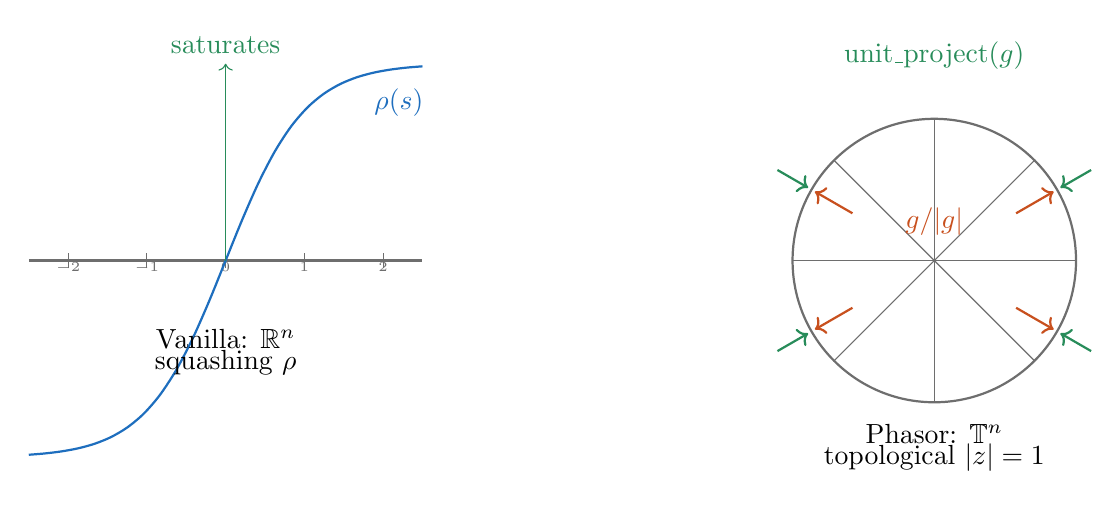
\begin{tikzpicture}[scale=1.0]
% LEFT: Real line with squashing
\begin{scope}[xshift=-4.5cm]
  \draw[axisgray, thick] (-2.5,0) -- (2.5,0);
  \foreach \x in {-2,-1,0,1,2} \draw[axisgray] (\x,-0.1) -- (\x,0.1) node[below,font=\tiny] {$\x$};
  % squashing curve
  \draw[holo, thick, domain=-2.5:2.5,smooth,variable=\x] plot ({\x},{2.5*tanh(\x)});
  \node[holo] at (2.2,2.0) {$\rho(s)$};
  \draw[->, probeC] (0,0) -- (0,2.5) node[above] {saturates};
  \node at (0,-1.0) {Vanilla: $\R^n$};
  \node at (0,-1.3) {squashing $\rho$};
\end{scope}

% RIGHT: Unit circle with projector
\begin{scope}[xshift=4.5cm]
  \draw[axisgray, thick] (0,0) circle (1.8);
  \foreach \ang in {0,45,...,315} \draw[axisgray, thin] (0,0) -- (\ang:1.8);
  % unit projector arrows (all pointing toward the unit circle)
  \foreach \ang in {30,150,210,330} {
    \draw[probeC, ->, thick] (\ang:2.3) -- (\ang:1.85);   % from outside
    \draw[antiholo, ->, thick] (\ang:1.2) -- (\ang:1.75); % from inside
  }
  \node[probeC] at (90:2.6) {$\unitproject(g)$};
  \node[antiholo] at (90:0.5) {$g/|g|$};
  \node at (0,-2.2) {Phasor: $\T^n$};
  \node at (0,-2.5) {topological $|z|=1$};
\end{scope}
\end{tikzpicture}
\caption{Vanilla activations live on a line with a squashing nonlinearity $\rho(s)$ that saturates. Phasors live on a circle; the unit projector $\unitproject(g)=g/|g|$ enforces $|z|=1$ as a topological constraint --- no saturating function, no bound to fight.}
\label{fig:statespace}
\end{figure}

\begin{figure}[ht]
\centering
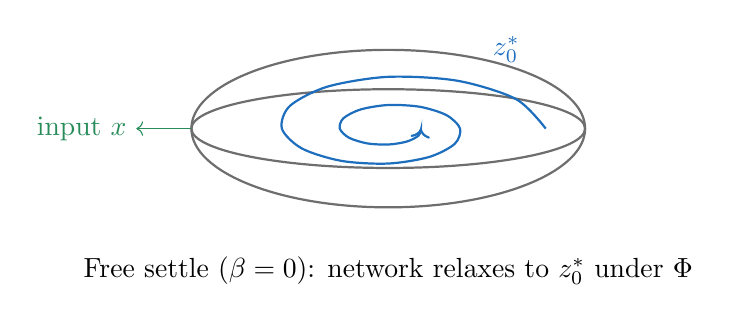
\begin{tikzpicture}[scale=1.0]
% Torus schematic with spiral trajectory
\begin{scope}
  % Torus surface (simplified as two circles)
  \draw[axisgray, thick] (0,0) ellipse (2.5 and 1.0);
  \draw[axisgray, thick] (0,0) ellipse (2.5 and 0.5);
  % Spiral trajectory
  \draw[holo, thick, ->] 
    plot[domain=0:4*pi,smooth,variable=\t] 
    ({2.0*exp(-\t/8)*cos(\t r)}, {0.8*exp(-\t/8)*sin(\t r)});
  \node[holo] at (1.5,1.0) {$z_0^*$};
  \draw[probeC, ->] (-2.5,0) -- (-3.2,0) node[left] {input $x$};
  \node at (0,-1.8) {Free settle ($\beta=0$): network relaxes to $z_0^*$ under $\Phi$};
\end{scope}
\end{tikzpicture}
\caption{Free settle trajectory on the torus. Starting from an initial condition, the network state spirals toward the free fixed point $z_0^*$ under the energy $\Phi$ with $\beta=0$. The unit projector keeps every neuron on the unit circle at each step.}
\label{fig:freesettle}
\end{figure}

%======================================================================
\section{The Non-Holomorphic Map and the AC Probe}\label{sec:problem}
%======================================================================

\subsection{The Fixed-Point Map}\label{ssec:fixed-point-map}

For a given input $x$, the network settles to a fixed point $z^*(\beta)$ that depends on the nudge $\beta$. In vanilla EP, this map $\beta \mapsto s_\beta^*$ is holomorphic, so a static real $\beta$ cleanly extracts the gradient via the two-phase contrast \citep{scellier2017equilibrium}. In the phasor case, the unit projector $\unitproject(g) = g/|g|$ depends explicitly on $\bar{g}$ --- it is not holomorphic. Consequently, the equilibrium $z^*(\beta)$ depends on both $\beta$ and $\bar{\beta}$. This non-holomorphicity is the fundamental reason LIEP differs from hEP \citep{laborieux2022holomorphic}.

\subsection{Linearization and Wirtinger Derivatives}\label{ssec:linearization}

For small $\beta$, we linearize the fixed-point map around the free equilibrium $z_0^*$:
\begin{equation}
z^*(\beta) \approx z_0^* + a\,\beta + b\,\bar{\beta},
\end{equation}
where the Wirtinger derivatives
\begin{equation}
a = \frac{\partial z^*}{\partial \beta}\Big|_{\beta=0},
\qquad
b = \frac{\partial z^*}{\partial \bar{\beta}}\Big|_{\beta=0}
\end{equation}
are both non-zero. The gradient of the loss with respect to the real-valued nudge is the sum
\begin{equation}
\frac{\dd z^*}{\dd \beta_R} = a + b.
\end{equation}
This is the quantity we need for learning.

\subsection{Frequency-Domain Picture}\label{ssec:frequency-picture}

Driving the system with a complex exponential $\beta(t) = \varepsilon e^{\im\omega_p t}$ produces a response containing both frequencies because the non-holomorphic map couples $\beta$ and $\bar{\beta}$. The linearized response is
\begin{equation}
z(t) - z_0^* \approx a\,\beta(t) + b\,\bar{\beta}(t) = a\varepsilon e^{\im\omega_p t} + b\varepsilon e^{-\im\omega_p t}.
\end{equation}
The holomorphic derivative $a$ appears at $+\omega_p$; the anti-holomorphic derivative $b$ appears at $-\omega_p$. A complex exponential at $-\omega_p$ swaps their roles.

\subsection{Why a Real Cosine Probe?}\label{ssec:why-ac}

A \emph{real cosine} $\beta(t) = \varepsilon \cos(\omega_p t) = \frac{\varepsilon}{2}(e^{\im\omega_p t} + e^{-\im\omega_p t})$ has equal energy at $\pm\omega_p$. Since $\cos$ is real, $\bar{\beta}(t) = \beta(t)$. The response becomes
\begin{equation}
z(t) - z_0^* \approx \frac{\varepsilon}{2}(a+b) e^{\im\omega_p t} + \frac{\varepsilon}{2}(a+b) e^{-\im\omega_p t} = \varepsilon(a+b)\cos(\omega_p t).
\end{equation}
Both Wirtinger components contribute \emph{coherently} at each sideband; the amplitude at $\pm\omega_p$ is proportional to $a+b$ — the real gradient we need.

A static $\beta$ is DC ($\omega=0$): both sidebands collapse to $\omega=0$ and sum to $a+b$ at DC. Extracting this requires two settles (free and nudged) to form a finite difference. The cosine probe keeps the sidebands separated in frequency; lock-in demodulation at $\omega_p$ recovers $a+b$ in a single settle.

\begin{figure}[ht]
\centering
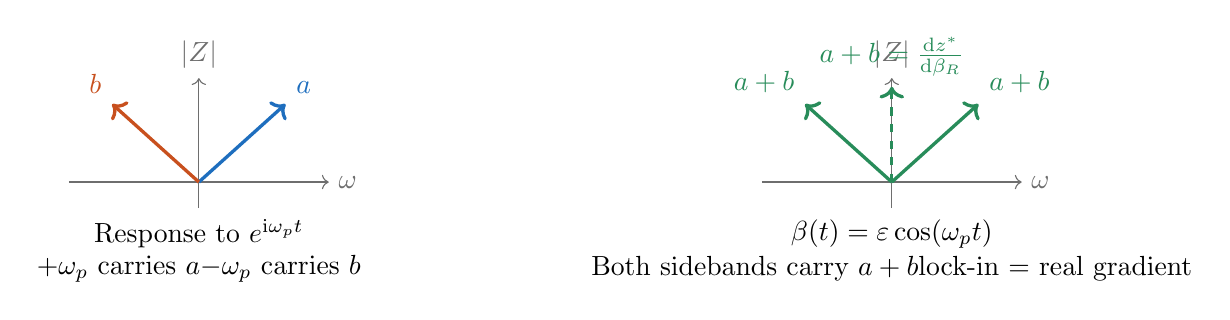
\begin{tikzpicture}[scale=1.1]
% LEFT: Sideband structure from complex exponential
\begin{scope}[xshift=-4cm]
  \draw[axisgray,->] (-1.5,0) -- (1.5,0) node[right] {$\omega$};
  \draw[axisgray,->] (0,-0.3) -- (0,1.2) node[above] {$|Z|$};
  \draw[holo, very thick, ->] (0,0) -- (1,0.9) node[above right] {$a$};
  \draw[antiholo, very thick, ->] (0,0) -- (-1,0.9) node[above left] {$b$};
  \node at (0,-0.6) {Response to $e^{\im\omega_p t}$};
  \node[align=center] at (0,-1.0) {$+\omega_p$ carries $a$\newline $-\omega_p$ carries $b$};
\end{scope}

% RIGHT: Real cosine probe — coherent sum at both sidebands
\begin{scope}[xshift=4cm]
  \draw[axisgray,->] (-1.5,0) -- (1.5,0) node[right] {$\omega$};
  \draw[axisgray,->] (0,-0.3) -- (0,1.2) node[above] {$|Z|$};
  \draw[probeC, very thick, ->] (0,0) -- (1,0.9) node[above right] {$a+b$};
  \draw[probeC, very thick, ->] (0,0) -- (-1,0.9) node[above left] {$a+b$};
  \draw[probeC, very thick, ->, dashed] (0,0) -- (0,1.1) node[above] {$a+b = \frac{\dd z^*}{\dd \beta_R}$};
  \node at (0,-0.6) {$\beta(t)=\varepsilon\cos(\omega_p t)$};
  \node[align=center] at (0,-1.0) {Both sidebands carry $a+b$\newline lock-in = real gradient};
\end{scope}
\end{tikzpicture}
\caption{Left: A complex exponential probe at $\omega_p$ separates the Wirtinger components: $+\omega_p$ carries $a$, $-\omega_p$ carries $b$. Right: A real cosine probe excites both frequencies equally; since $\beta=\bar{\beta}$, both sidebands carry the coherent sum $a+b$. Lock-in demodulation at $\omega_p$ extracts the real gradient in one settle.}
\label{fig:sideband-comparison}
\end{figure}

%======================================================================
\section{The Lock-in Solution: Real AC Probe}\label{sec:lockin}
%======================================================================

The remedy is to drive the nudge as a small real cosine in time,
\begin{equation}
\beta(t) = \varepsilon \cos(\omega_p t),
\end{equation}
applied \emph{only at the output layer}, with $\varepsilon \ll 1$. The network oscillates around the free fixed point $z_0^*$ at frequency $\omega_p$; no second phase is needed.

\subsection{From State Response to Weight Gradient}\label{ssec:state-to-gradient}

The energy function is
\begin{equation}
\Phi = \sum_{\ell=1}^L \Real\langle W_\ell z_{\ell-1}, z_\ell \rangle - \beta\, C(z_L, y).
\end{equation}
Its derivative with respect to the weights gives the gradient we need for learning:
\begin{equation}
\frac{\partial \Phi}{\partial W_\ell} = \Real\big( z_\ell z_{\ell-1}^H \big) \;\equiv\; H_\ell.
\end{equation}
This is the local Hebbian quantity — the phase alignment between the post-synaptic state $z_\ell$ and the pre-synaptic state $z_{\ell-1}$.

When we inject the probe $\beta(t) = \varepsilon\cos(\omega_p t)$, the states oscillate around the free fixed point:
\begin{equation}
z_\ell(t) \approx z_{\ell,0}^* + \delta z_\ell(t),
\end{equation}
where $\delta z_\ell(t)$ is proportional to $\varepsilon$ and oscillates at $\omega_p$ (in the linear regime).

Substitute into the Hebbian:
\begin{align}
H_\ell(t) &= \Real\big( z_\ell(t) z_{\ell-1}(t)^H \big) \\
&\approx \Real\big( (z_{\ell,0}^* + \delta z_\ell(t)) (z_{\ell-1,0}^* + \delta z_{\ell-1}(t))^H \big) \\
&= H_{\ell,0} + \Real\big( \delta z_\ell(t) z_{\ell-1,0}^{*H} + z_{\ell,0}^* \delta z_{\ell-1}(t)^H \big) + O(\varepsilon^2).
\end{align}
The oscillating part $\delta H_\ell(t) = H_\ell(t) - H_{\ell,0}$ is proportional to $\varepsilon$ and oscillates at $\omega_p$. In the linear regime, its amplitude is proportional to the energy gradient $\partial\Phi/\partial W_\ell$. Specifically:
\begin{equation}
\delta H_\ell(t) \approx \frac{\varepsilon}{2}\,\frac{\partial \Phi}{\partial W_\ell}\,\cos(\omega_p t).
\end{equation}

Lock-in demodulation extracts this amplitude: multiply by $\cos(\omega_p t)$ and average over integer periods $T = 2\pi/\omega_p$:
\begin{align}
\langle H_\ell \rangle_{\omega_p}
&= \frac{2}{T}\int_0^T H_\ell(t) \cos(\omega_p t) \, \dd t \\
&\approx \frac{2}{T}\int_0^T \Big[ H_{\ell,0} + \frac{\varepsilon}{2}\frac{\partial \Phi}{\partial W_\ell}\cos(\omega_p t) \Big] \cos(\omega_p t) \, \dd t \\
&= \frac{\varepsilon}{2}\frac{\partial \Phi}{\partial W_\ell} \cdot \frac{2}{T}\int_0^T \cos^2(\omega_p t) \, \dd t \\
&= \frac{\varepsilon}{2}\frac{\partial \Phi}{\partial W_\ell}.
\end{align}
We used $\int_0^T \cos^2(\omega_p t) \dd t = T/2$ and the DC term $H_{\ell,0}\cos(\omega_p t)$ averages to zero.

The EP theorem states that the loss gradient is the $\beta$-derivative of the energy gradient \citep{scellier2017equilibrium,scellier2018equivalence}:
\begin{equation}
\frac{\partial \mathcal{L}}{\partial W_\ell} = \lim_{\beta\to 0} \frac{1}{\beta}\Big[
\frac{\partial \Phi}{\partial W_\ell}\big|_{z_\beta^*} - \frac{\partial \Phi}{\partial W_\ell}\big|_{z_0^*}
\Big].
\end{equation}
The lock-in demodulation approximates this finite difference using the AC probe amplitude. Since $a+b = \dd z^*/\dd\beta_R$ and $\partial\mathcal{L}/\partial W_\ell = -(a+b)$ (minus sign from $\Phi = E - \beta C$), we obtain:
\begin{equation}
\frac{\partial \mathcal{L}}{\partial W_\ell} \approx - (a+b) = -\frac{2}{\varepsilon} \langle H_\ell \rangle_{\omega_p}.
\end{equation}

\subsection{The Lock-in Gradient Formula}

At each layer, the local Hebbian quantity
\begin{equation}
H_\ell(t) = \Real\big( z_\ell(t) \, z_{\ell-1}(t)^H \big)
\end{equation}
oscillates at $\omega_p$. Lock-in demodulation extracts its $\omega_p$ component: multiply by $\cos(\omega_p t)$ and average over an integer number of periods $T = 2\pi/\omega_p$:
\begin{equation}
\langle H_\ell \rangle_{\omega_p} = \frac{2}{T}\int_0^T H_\ell(t) \cos(\omega_p t) \, \dd t.
\end{equation}
In the linear regime, this yields the gradient with respect to the weights. The resulting per-layer update is

\begin{equation}\boxed{
\frac{\partial \mathcal{L}}{\partial W_\ell}
\;=\;
-\frac{2}{\varepsilon}\,
\Big\langle \Real\big(z_\ell z_{\ell-1}^H\big)\;\cos(\omega_p t) \Big\rangle_T
}\label{eq:lockin-gradient}
\end{equation}

where the average is over integer cycles of the probe. The factor $2/\varepsilon$ normalizes the probe amplitude. Crucially, this is a \emph{local} learning rule: the gradient for $W_\ell$ requires only the pre-synaptic state $z_{\ell-1}$ and post-synaptic state $z_\ell$ at the same layer, plus the globally broadcast probe $\cos(\omega_p t)$. No error signal is backpropagated. This locality property is shared with the original EP \citep{scellier2017equilibrium} and is a key motivation for neuromorphic implementations \citep{ororbia2023brain,whittington2019theories}.

\begin{figure}[ht]
\centering
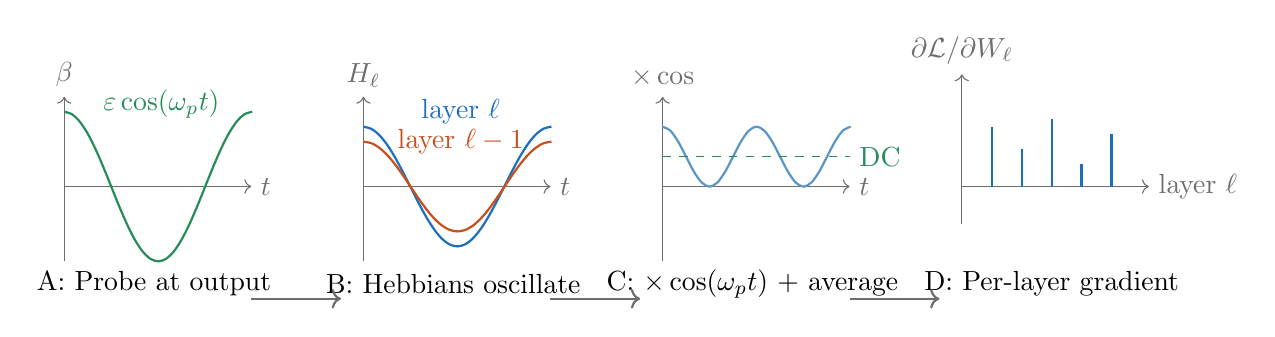
\begin{tikzpicture}[scale=0.95]
% Panel A: Probe injection
\begin{scope}[xshift=-6.5cm, yshift=0]
  \draw[axisgray,->] (0,0) -- (2.5,0) node[right] {$t$};
  \draw[axisgray,->] (0,-1) -- (0,1.2) node[above] {$\beta$};
  \draw[probeC, thick, domain=0:2*pi,smooth,variable=\t] plot ({\t/2.5},{cos(\t r)});
  \node[probeC] at (1.3,1.1) {$\varepsilon\cos(\omega_p t)$};
  \node at (1.2,-1.3) {A: Probe at output};
\end{scope}

% Panel B: Network oscillation
\begin{scope}[xshift=-2.5cm, yshift=0]
  \draw[axisgray,->] (0,0) -- (2.5,0) node[right] {$t$};
  \draw[axisgray,->] (0,-1) -- (0,1.2) node[above] {$H_\ell$};
  \draw[holo, thick, domain=0:2*pi,smooth,variable=\t] plot ({\t/2.5},{0.8*cos(\t r + 0.3)});
  \draw[antiholo, thick, domain=0:2*pi,smooth,variable=\t] plot ({\t/2.5},{0.6*cos(\t r - 0.2)});
  \node[holo] at (1.3,1.0) {layer $\ell$};
  \node[antiholo] at (1.3,0.6) {layer $\ell-1$};
  \node at (1.2,-1.3) {B: Hebbians oscillate};
\end{scope}

% Panel C: Demodulation
\begin{scope}[xshift=1.5cm, yshift=0]
  \draw[axisgray,->] (0,0) -- (2.5,0) node[right] {$t$};
  \draw[axisgray,->] (0,-1) -- (0,1.2) node[above] {$\times\cos$};
  \draw[basinC, thick, domain=0:2*pi,smooth,variable=\t] plot ({\t/2.5},{0.8*cos(\t r + 0.3)*cos(\t r)});
  \draw[probeC, dashed] (0,0.4) -- (2.5,0.4) node[right] {DC};
  \node at (1.2,-1.3) {C: $\times\cos(\omega_p t)$ + average};
\end{scope}

% Panel D: Gradient
\begin{scope}[xshift=5.5cm, yshift=0]
  \draw[axisgray,->] (0,0) -- (2.5,0) node[right] {layer $\ell$};
  \draw[axisgray,->] (0,-0.5) -- (0,1.5) node[above] {$\partial\mathcal{L}/\partial W_\ell$};
  \foreach \i/\val in {1/0.8, 2/0.5, 3/0.9, 4/0.3, 5/0.7} {
    \draw[holo, thick] (\i*0.4,0) -- (\i*0.4,\val);
  }
  \node at (1.2,-1.3) {D: Per-layer gradient};
\end{scope}

% Arrows between panels
\draw[->, thick, axisgray] (-4.0,-1.5) -- (-2.8,-1.5);
\draw[->, thick, axisgray] (0.0,-1.5) -- (1.2,-1.5);
\draw[->, thick, axisgray] (4.0,-1.5) -- (5.2,-1.5);
\end{tikzpicture}
\caption{Lock-in EP in one settle. (A) Real cosine probe $\varepsilon\cos(\omega_p t)$ injected at output. (B) Network oscillates; each layer's Hebbian $H_\ell = \Real(z_\ell z_{\ell-1}^H)$ oscillates at $\omega_p$. (C) Multiply by $\cos(\omega_p t)$ and average over integer cycles $T$ extracts the DC component. (D) Result: gradient $\partial\mathcal{L}/\partial W_\ell$ for each layer. No second phase, no backpropagation.}
\label{fig:timeline}
\end{figure}

%======================================================================
\section{Operating Regime}\label{sec:operating-regime}
%======================================================================

LIEP has three primary control knobs that must be balanced for reliable gradient estimation:

\begin{table}[ht]
\centering
\caption{LIEP operating knobs.}
\label{tab:knobs}
\begin{tabular}{@{}lll@{}}
\toprule
Knob & Symbol & Role \\
\midrule
Probe amplitude & $\varepsilon$ & Linear regime vs. basin hopping \\
Probe frequency & $\omega_p$ & Adiabaticity vs. settling speed \\
Integration cycles & $T_{\text{int}}$ & Demodulator selectivity vs. latency \\
\bottomrule
\end{tabular}
\end{table}

\paragraph{Adiabaticity ($\omega_p \ll R_{\text{relax}}$).}
The probe frequency must be much slower than the network's relaxation rate $R_{\text{relax}}$ (the inverse settling time). If $\omega_p$ is too high, the network cannot track the probe and the linear response assumption breaks down. In practice, $\omega_p \sim 0.1$--$0.5 \times R_{\text{relax}}$ works well.

\paragraph{Probe amplitude ($\varepsilon$).}
Too small: gradient signal buried in numerical noise. Too large: nonlinear response, basin hopping (the probe kicks the state out of the free fixed point's basin of attraction). The sweet spot is $\varepsilon \sim 10^{-3}$--$10^{-2}$ for typical weight scales. Basin hopping is more likely when $\varepsilon / \|W\| \gtrsim 0.1$.

\paragraph{Integration cycles ($T_{\text{int}}$).}
The lock-in integral runs over $T_{\text{int}}$ cycles of the probe. Larger $T_{\text{int}}$ gives better harmonic rejection but increases latency. $T_{\text{int}} = 4$--$8$ cycles is typical.

\paragraph{Self-energy mode ($K_{\text{mode}}$).}
$K_{\text{mode}}=:\text{zero}$ (default) omits the self-energy term; the decay comes purely from $(1-\dt)z$. $K_{\text{mode}}=:\text{stored}$ adds the per-channel $\lambda$ decay from $\log\_neg\_lambda$. The latter can speed up settling but requires smaller $\dt$ or soft projection to avoid instability. This connects to dense associative memory models \citep{krotov2016dense} where self-interaction shapes the energy landscape.

\paragraph{Rotating frame / carrier.}
The exact carrier rotation (§\ref{ssec:rotating-frame}) makes LIEP equivalent in the co-rotating and lab frames at any $\dt$. For spiking deployment, the physical carrier frequency $\omega$ is a hardware parameter; the learning dynamics are frame-invariant.

\paragraph{Quantization dead zone.}
At spike-time readout, phases are quantized to spike times. Very small phase differences (below $\sim 2\pi / N_{\text{spikes}}$) fall into a dead zone where the gradient signal is lost. This limits the effective precision of the gradient at small $\varepsilon$.

%======================================================================
\section{Honest Scope \& Limitations}\label{sec:scope}
%======================================================================

\paragraph{What works (empirically validated).}
\begin{itemize}
\item Depth 2 networks (one hidden layer) with $K_{\text{mode}}=:\text{zero}$.
\item FashionMNIST classification: $\sim 84\%$ test accuracy (comparable to BP baseline).
\item Local learning rule: gradients match finite-difference to $\sim 2\%$ relative error.
\item Both atemporal (discrete) and spiking (ODE) execution modes.
\end{itemize}

\paragraph{What does not work (known failure modes).}
\begin{itemize}
\item Depth $\ge 3$: gradients degrade exponentially with depth; the phase-locked carrier assumption breaks down as feedback signals accumulate phase noise.
\item $K_{\text{mode}}=:\text{stored}$ at scale: per-channel $\lambda$ introduces additional dissipation that couples with the probe, causing instability unless $\dt \ll 0.5$ and soft projection are used.
\item Asymmetric feedback: LIEP assumes symmetric feedback ($W_{\ell+1}^\top$) for the energy gradient. Asymmetric feedback (e.g., random backward weights) breaks the EP theorem; gradients no longer match the loss \citep{scellier2017equilibrium}.
\item Binding in energy: The VSA binding operation (elementwise phase addition) is not represented in the energy $\Phi$; it is a readout-time operation only \citep{olin2023hyperdimensional}.
\item Large batch sizes with carrier: the shared carrier across batches assumes identical frequency; batch-level frequency drift is not modeled.
\end{itemize}

\paragraph{Theoretical gaps.}
\begin{itemize}
\item No convergence proof for the discrete dynamics with hard projection at finite $\dt$.
\item The linear response regime ($\varepsilon \to 0$) is not rigorously connected to the finite-$\varepsilon$ lock-in gradient.
\item Rotating frame equivalence assumes exact U(1) covariance of the drive; this holds for the energy gradient but not for all possible cost functions.
\item Quantization effects at spike-time readout are not incorporated into the energy landscape.
\end{itemize}

\paragraph{Hardware considerations.}
LIEP is designed for neuromorphic substrates where:
\begin{itemize}
\item The probe $\varepsilon\cos(\omega_p t)$ is a physical AC current injected at the output.
\item Lock-in demodulation is implemented by analog multipliers and integrators (or digital correlators).
\item The local Hebbian $H_\ell = \Real(z_\ell z_{\ell-1}^H)$ maps to a spike-timing-dependent plasticity (STDP) window.
\end{itemize}
The three-factor STDP formulation (pre $\times$ post $\times$ global probe) is derived in the companion proof and matches the biological three-factor learning rule hypothesis \citep{ororbia2023brain}.

%======================================================================
\appendix
\section{Full Derivation: LIEP Energy and Settling}\label{sec:liep_proof}
%======================================================================

This appendix provides the complete Wirtinger-derivative derivation of the energy gradient and the projected settling dynamics. For expanded proofs (tangent projection equivalence, rotating frame, soft projection, non-holomorphic map linearization), see the companion proof document \texttt{liep\_companion\_proof.tex}.

\subsection{Wirtinger Derivative of the Layer Energy}

The layer energy is $\Phi_\ell = \Real\langle W_\ell z_{\ell-1}, z_\ell \rangle = \frac{1}{2}(z_\ell^H W_\ell z_{\ell-1} + z_{\ell-1}^H W_\ell^T z_\ell)$. Since $W_\ell$ is real, $W_\ell^T = W_\ell^\top$. The Wirtinger derivative with respect to $\bar{z}_\ell$ (holding $z_\ell$ constant) is
\begin{equation}
\frac{\partial \Phi_\ell}{\partial \bar{z}_\ell} = \frac{1}{2} W_\ell z_{\ell-1}.
\end{equation}
Similarly, $\Phi_{\ell+1} = \Real\langle W_{\ell+1} z_\ell, z_{\ell+1} \rangle$ gives
\begin{equation}
\frac{\partial \Phi_{\ell+1}}{\partial \bar{z}_\ell} = \frac{1}{2} W_{\ell+1}^\top z_{\ell+1}.
\end{equation}
Summing both contributions (the layer $\ell$ state appears in two coupling terms) yields
\begin{equation}
\frac{\partial \Phi}{\partial \bar{z}_\ell} = \frac{1}{2}\big( W_\ell z_{\ell-1} + W_{\ell+1}^\top z_{\ell+1} \big) + \frac{1}{2}\big( W_\ell z_{\ell-1} + W_{\ell+1}^\top z_{\ell+1} \big) = W_\ell z_{\ell-1} + W_{\ell+1}^\top z_{\ell+1}.
\end{equation}
For the output layer $\ell=L$, the cost term $C = 1 - \frac{1}{d}\Real\langle z_L, y \rangle$ contributes $-\beta\, \frac{\partial C}{\partial \bar{z}_L} = \frac{\beta}{2d} y + \frac{\beta}{2d} y = \frac{\beta}{d} y$, giving~\eqref{eq:grad-output}.

\subsection{Decay Term Origin}

The term $-z_\ell$ in~\eqref{eq:continuous-flow} is a linear decay added for stability; it is \emph{not} a gradient of the energy $\Phi$. The energy provides only the coupling forces between layers. The continuous-time dynamics with explicit decay are
\begin{equation}
\frac{\dd z_\ell}{\dd t} = -\gamma z_\ell - \frac{\partial \Phi}{\partial \bar{z}_\ell},
\end{equation}
and setting $\gamma = 1$ recovers~\eqref{eq:continuous-flow}. In the discrete settle~\eqref{eq:discrete-settle-impl}, this decay appears as the $(1-\dt)z_\ell$ term (explicit convex combination), and is the form used in all experiments (`K_mode=:zero` in \texttt{src/ep.jl}).

\subsection{Projected Euler Justification}

The continuous flow~\eqref{eq:continuous-flow} preserves $|z|$ only if the velocity is tangent to the torus. The projected Euler method:
\begin{enumerate}
\item Takes an Euler step in the ambient space: $\tilde{z} = z + \dt\, v$,
\item Projects back: $z_+ = \unitproject(\tilde{z})$.
\end{enumerate}
For small $\dt$, this is equivalent to projecting $v$ onto the tangent space $T_z\T^n$ and flowing along the geodesic. The tangent projection of $v \in \C^n$ is $v - \Real(\bar{z} \odot v) \odot z$ (entrywise), which for $v = -z + \text{drive}$ gives the same first-order update as the simple normalization. The discrete update~\eqref{eq:discrete-settle-impl} is therefore a consistent first-order integrator for the constrained gradient flow on $\T^n$.

%======================================================================
\section{Bibliography}\label{sec:bibliography}
%======================================================================

\bibliographystyle{plainnat}
\bibliography{liep_companion_proof}

\end{document}